\documentclass[11pt,a4paper]{article}

\usepackage[T1]{fontenc}
\usepackage[utf8]{inputenc}
\usepackage{amsmath,amssymb}
\usepackage{graphicx}
\usepackage{booktabs}
\usepackage{tabularx}
\usepackage{ragged2e}
\usepackage{natbib}
\usepackage{url}
\usepackage{hyperref}
\usepackage{lineno}
\usepackage{geometry}
\usepackage{caption}
\usepackage[protrusion=true,expansion=false]{microtype}

\geometry{margin=2.5cm}
\linenumbers
\pagestyle{plain}

% natbib author-year setup
\bibpunct{(}{)}{;}{a}{,}{,}

% upright derivative d
\newcommand{\diff}{\mathrm{d}}

\title{Beyond Binary Lock: A Continuous Aperture-Collapse Hazard Model of Middle-Ear Barotrauma in Hypobaric-Chamber Training}

\author{%
  Diego L. Malpica\thanks{Corresponding author. Email: \href{mailto:diego.malpica@fac.mil.co}{diego.malpica@fac.mil.co}. ORCID: \href{https://orcid.org/0000-0002-2257-4940}{0000-0002-2257-4940}.}\,$^{1,2}$
  \and Marian A. Farf\'{a}n\thanks{ORCID: \href{https://orcid.org/0000-0002-9910-6053}{0000-0002-9910-6053}.}\,$^{1}$%
}

\date{%
\small
$^{1}$Subdirectorate of Aerospace Sciences, Direction of Aerospace Medicine (DIMAE), Colombian Aerospace Force, Bogot\'{a}, Colombia.\\[2pt]
$^{2}$Aerospace Medicine Research Program, DIMAE, Colombian Aerospace Force, Bogot\'{a}, Colombia.%
}


\begin{document}

\maketitle

\begin{abstract}
\textbf{Background.} Middle-ear barotrauma (MEB) is the most common complication of pressurised flight and hypobaric-chamber training, and a proxy for Eustachian-tube disease that disqualifies aviator candidates. Kanick-Doyle's 2005 model reproduces airline-descent physiology but does not address chamber descent rates of 1,000--10,000 ft$\cdot$min$^{-1}$, treats Patulous Eustachian tube (PET) as rupture-protective, and does not parameterise acute upper-respiratory-infection (URI) modifiers despite URI dominance as a modifiable risk factor.

\textbf{Objective.} To develop and externally validate a physics-informed, pathophysiology-aware prediction model for per-exposure MEB risk during hypobaric-chamber training.

\textbf{Methods.} We extended Kanick-Doyle with (i) a continuous descent-side aperture-collapse function (Hill function with rate-dependent tightening), (ii) a six-state URI temporal modifier table, (iii) a four-state PET model, (iv) a lumped-parameter approximation of Ghadiali-group muscle mechanics, and (v) a three-threshold cumulative-hazard score. No machine-learning component is used. Hazard constants were calibrated to the pooled Colombian Aerospace Force (FAC) DIMAE 2010--2026 registry (173/7,271; 2.38\% per-exposure) via log-space bisection and Approximate Bayesian Computation Sequential Monte Carlo (ABC-SMC). External validation used three previously published military-aviation cohorts \citep{Morgagni2012,Landolfi2009,Morgagni2010} without parameter refitting.

\textbf{Results.} Calibration reproduced the pooled FAC anchor within 0.1 pp (simulated 2.47\%; career-3 projection 7.23\% vs. 6.97\%). External validation fell inside the observed Wilson 95\% confidence interval for two of three benchmarks (3.31\% vs. 2.3\% [1.13\%, 4.62\%]; 3.37\% vs. 2.4\% [1.22\%, 4.66\%]); the third cohort's gap (+1.77 pp) matched its own pre-/unscreened denominator spread. Saltelli-Sobol sensitivity identified the aperture half-point as the dominant variance driver.

\textbf{Conclusion.} The model reproduces operational MEB prevalence and transfers across independent military-aviation cohorts without refitting. Open-source simulator: \url{https://github.com/strikerdlm/barotrauma_model}

\textbf{Keywords:} Eustachian tube dysfunction; altitude training; upper respiratory infection; physics-informed modelling; external validation.
\end{abstract}

\section{Introduction}

Middle-ear barotrauma (MEB) --- the inability of the Eustachian tube (ET) to equalize middle-ear pressure against changing ambient pressure --- affects an estimated 3--10\% of aircrew per hypobaric-chamber exposure \citep{Morgagni2012,Landolfi2009,Morgagni2010} and up to 85\% of commercial aircrew over their careers \citep{Lindfors2021}. In military aviation medicine its importance is twofold: as a direct medical consequence of altitude training, and as a proxy for the broader spectrum of Eustachian-tube disease that disqualifies aviator applicants and restricts operational employment.

The most widely used mathematical description is Kanick and Doyle's 2005 pressure-regulation model \citep{Kanick2005}. Their gas-exchange framework combines Boyle's-law tympanic-membrane buffering, Hagen-Poiseuille bulk flow through an intermittently opening Eustachian tube, swallow-driven active openings with a fixed muscular resistance $R_A$, and trans-mucosal species diffusion. The model reproduces passenger airline physiology accurately and is the reference against which subsequent work is benchmarked. Three shortcomings limit its direct use in hypobaric-chamber decision support.

First, chamber training descent rates of 1,000--10,000 ft$\cdot$min$^{-1}$ exceed cabin descent by a factor of 5--30. At these rates the developing intra-tubal pressure gradient progressively collapses the collapsible cartilaginous portion of the ET, a Hagen-Poiseuille r$^{4}$ effect that Kanick-Doyle's binary "open or locked" treatment approximates but does not resolve continuously. Second, Kanick-Doyle model obstructive dysfunction through $R_A$ and Patulous ET through a trivial "always open" case that predicts complete rupture protection. Clinical experience contradicts the latter when mucosal edema (such as concurrent URI) converts a patent tube into a paradoxically closed one \citep{Kobayashi2018,Kikuchi2017,Shindo2025}. Third, controlled rhinovirus-challenge data have documented substantial ET dysfunction persisting for 2--3 weeks post-onset \citep{McBride1989,Buchman1994,Doyle1999}, and survey data show URI to be the dominant modifiable risk factor for MEB in flying populations \citep{Lindfors2021,Boel2017}, yet the Kanick-Doyle parameters do not vary with URI state.

We present a physics-informed, pathophysiology-aware extension that addresses these gaps, calibrated to the Colombian Aerospace Force (FAC) 10-year operational registry and externally validated on three independent previously published military-aviation cohorts. The software is released open-source at \url{https://github.com/strikerdlm/barotrauma_model} under the MIT license.



\section{Methods}

\subsection{2.1 Study design, reporting, and ethics}

This is a computational prediction-model study comprising model development followed by external validation on three independent, previously published cohorts. Reporting follows the TRIPOD 2015 guideline (Transparent Reporting of a multivariable prediction model for Individual Prognosis Or Diagnosis); the completed 28-item checklist is provided as Supplementary File S1. No machine-learning component is used in the deployed prediction pipeline; the sklearn scaffolding referenced in the source repository is disabled and does not alter the deterministic physics output. TRIPOD+AI (2024) therefore does not apply.

Under Colombian Resolution 8430 of 1993 of the Ministry of Health (\textit{Ministerio de Salud, "Por la cual se establecen las normas científicas, técnicas y administrativas para la investigación en salud"}), Article 11(a), research that uses retrospective documentary methods and de-identified records --- without intervention or modification of biological, physiological, psychological, or social variables of subjects --- is classified as \textbf{\textit{investigación sin riesgo}} (research without risk) and does not require institutional-ethics-committee submission or individual informed consent. The present study meets these criteria: data are retrospective, de-identified prior to analysis, and no intervention was performed. The study was conducted in accordance with the principles of the Declaration of Helsinki (2013 revision). Calibration is anchored to aggregate institutional statistics only. \textbf{Publication of this work was authorized by the Colombian Aerospace Force.}

\subsection{2.2 Model architecture}

The simulator is implemented in pure Python (NumPy and SciPy) as the \texttt{barotrauma.v2} package. It takes as inputs a patient state (anatomy, ET function, URI state, PET state, chronic rhinitis, medications, behavior) and a piecewise-linear chamber profile (ascent, hold, descent, or rapid-decompression segments). Output is a time-domain trace ($\Delta P$, tympanic-membrane displacement, ET open-closed raster, swallow and Valsalva timestamps) and per-outcome probabilities scored by a dose-response hazard model.

\subsection{2.3 Physics core}

The physics core retains the Kanick-Doyle 2005 structure: standard-atmosphere altitude-to-pressure map P(z) = P$_{0}$ exp(-z/H) with H = 29,921 ft; two-compartment middle-ear volume $V_{\mathrm{ME}}$ = $V_{\mathrm{tympanum}}$ + $V_{\mathrm{mastoid}}$ with the mastoid drawn from a log-normal prior (median 7.0 mL, 95\% interval 2.9--16.9 mL) matching \citet{Alper2011}; tympanic-membrane volume displacement clamped at $\pm$0.025 mL (1\% of $V_{\mathrm{ME}}$, Kanick-Doyle Table 1); passive ME-side ET opening when $\Delta P$ > 25.7 mmHg venting to 7.35 mmHg; active swallow-driven openings at a descent-phase frequency of 60$\cdot$hr$^{-1}$ (trained aircrew default; Kanick-Doyle's 31$\cdot$hr$^{-1}$ passive baseline is available as an override), each clearing a Fractional Gradient Equalized of 0.32, set to the upper bound of the 95\% CI 0.18--0.34 reported for adult ears with no significant otitis-media history \citep{Doyle2014}; Valsalva pulses every 60 s on descent with per-pulse clearance 0.55; an ET-lock state at |$\Delta P$| > 90 mmHg tightened by inflammation; species-resolved trans-mucosal Fick exchange with $\mathrm{O}_2$, $\mathrm{CO}_2$, $\mathrm{N}_2$, and $\mathrm{H}_2\mathrm{O}$ rate constants from \citep{Doyle2011}.

\subsection{2.4 Descent-side aperture-collapse model}

The central physical insight is that active ET clearance pathways (swallow and Valsalva) are progressively defeated during descent because the nasopharyngeal tissue pressure compresses the cartilaginous lumen from the NP side. We model this with a continuous aperture factor $\alpha$($\Delta P$, $\mathrm{d}\Delta P/\mathrm{d}t$) $\in$ [0, 1] applied multiplicatively to the per-event Fractional Gradient Equalized. For $\Delta P$ $\geq$ 0 (ascent) $\alpha$ = 1; for descent, $\alpha$ = 1 below a 40-mmHg free zone, then decays as 1 / (1 + ((|$\Delta P$| - free\_zone) / ($\Delta P_{1/2}$ - free\_zone))$^{n}$) with $\Delta P_{1/2}$ = 110 mmHg and n = 3. A rate-tightening factor 1 + 0.15 $\cdot$ min(rate, 3 mmHg$\cdot$s$^{-1}$) reduces effective $\Delta P_{1/2}$ under fast ambient-pressure changes, reflecting mucosal viscoelastic lag. An inflammation-tightening factor $\surd$($R_A$-multiplier) additionally narrows the threshold under URI. The aperture factor applies to active swallows at unit power and to Valsalva pulses at square-root power --- the muscular push of Valsalva partially overrides progressive collapse.

\subsection{2.5 Pathophysiology state machine}

URI state is encoded as one of six day-windows (none, 1--3, 4--7, 8--14, 15--21, 22--28), each with a tabulated multiplier set (Table~\ref{tab:uri_modifiers}). Multipliers were derived from controlled rhinovirus-challenge data \citep{McBride1989,Buchman1994,Doyle1999} and ETDQ-7 meta-analyses \citep{Chen2022}. The peak-dysfunction window (days 4--7) carries $R_A$ $\times$ 3.5, $P_O'$ shift +150 daPa (+11.3 mmHg), a 50\% drop in equalization-rate modifier, and a 4.25$\times$ per-descent MEB relative-risk multiplier.

Patulous ET (PET) is encoded as one of four states \citep{Kobayashi2018,Kikuchi2017,Shindo2025}. S1 (baseline patent, upright, dry mucosa) reproduces Kanick-Doyle's rupture-protective prediction via a hard-zero override on $\Delta P$. S2 (PET with acute URI or mucosal inflammation) applies paradoxical closure on an abnormal cartilaginous substrate via $R_A$ $\times$ 3.5, $P_O'$ shift +60 daPa, and a 4.0$\times$ per-descent RR. S3 (habitual sniffer) biases resting $\Delta P$ toward -15 mmHg, reflecting the type-B/C tympanogram rate of 42.6\% reported in habitually-sniffing PET patients \citep{Shindo2025}. Per-descent RR was raised from 2.5 to 4.0 to reflect the \citet{Oshima2025} large-cohort (n = 1,009) sniffing OR of 8.18 convolved with the already-modeled $\Delta P$ physiology. S4 (post-Kobayashi-plug or cartilage augmentation) imposes stenotic-equivalent obstruction. Oral and topical decongestants carry a paradoxical-worsening RR of 1.4 in PET (versus 0.90 in healthy subjects --- softened from the prior 0.70 per \citet{Moayedi2025}, a placebo-controlled HBOT RCT showing null preventive effect of prophylactic pseudoephedrine).

\subsection{2.6 Muscle mechanics and multi-pathway gas exchange}

A lumped-parameter approximation of Ghadiali-group FEM and multi-scale work \citep{Ghadiali2004} captures three time-dependent muscle effects on per-swallow FGE without running a full 2-D or 3-D FEM per integration step: fatigue and priming (recent swallows boost FGE up to +15\% with $\tau$ $\approx$ 8 s), mucosal adhesion buildup (prolonged closure at high |$\Delta P$| raises intraluminal surface tension with $\tau$ $\approx$ 30 s), and TVP/LVP timing variability (stochastic multiplier CV 5\% healthy, 15\% dysfunctional). The extension is disabled by default. The trans-mucosal Fick diffusion is extended with trans-TM (~4\% of mucosa rate) and trans-round-window (~1\%) pathways per \citep{Doyle2017}.

\subsection{2.7 Three-threshold hazard model}

Per-outcome probabilities are scored by a cumulative hazard applied to the $\Delta P$ trajectory: $h_i(t)$ = $r_i$ $\cdot$ max(0, |$\Delta P$(t)| - $\Theta_i)^{n_i}$ with $P_i$ = 1 - exp(-$\int$ $h_i$ dt). Thresholds align with Kanick-Doyle's clinical values: barotitis onset $\Theta$ = 18.4 mmHg (250 mmH$_{2}$O, n = 1.8); baromyringitis $\Theta$ = 95.6 mmHg (1,300 mmH$_{2}$O, n = 2.5); rupture $\Theta$ = 150 mmHg (conservative, n = 3). Per-stratum probabilities are multiplied by the composite per-descent RR (URI $\times$ PET $\times$ rhinitis $\times$ medication $\times$ history).

\subsection{2.8 Calibration and external validation}

\textbf{Source of data and participants (development cohort).} The development dataset comprises all hypobaric-chamber training exposures recorded in the DIMAE registry between 1 January 2010 and 31 March 2026 (n = 7,271 exposures) performed by active-duty and reserve military aviators and aircrew of the Colombian Aerospace Force at the DIMAE hypobaric chamber facility (Bogotá, 2,640 m elevation). Eligibility was operational --- all aircrew and aviator candidates scheduled for periodic or qualifying altitude indoctrination --- with no exclusion by age, sex, or prior ear history.

\textbf{Outcome.} The primary outcome was clinically diagnosed middle-ear barotrauma (Teed grade $\geq$ I) occurring during or within 24 hours of a chamber exposure, ascertained by the on-duty chamber flight surgeon using otoscopic, tympanometric, and symptomatic criteria. A total of 173 barotrauma events were recorded in the 7,271 exposures (per-exposure rate 2.38\%; Wilson 95\% CI, 2.06\%--2.75\%; projected 3-exposure career rate 6.97\%).

\textbf{Predictors.} Candidate predictors entering the model were: descent rate and altitude profile segment; mastoid volume (log-normal prior); Eustachian-tube resistance $R_A$ and passive opening pressure $P_O'$; URI temporal state (6 levels); PET state (4 levels); chronic rhinitis; decongestant use; prior MEB history; and swallow and Valsalva frequency. No variable selection was performed; the model is mechanistic and retains all predictors by construction.

\textbf{Missing data.} No imputation was performed because the anchor is an aggregate population statistic (count of events / count of exposures); individual-level missingness is absorbed in the cohort prior and the synthetic cohort sampling.

\textbf{Calibration methods.} Calibration used two methods. Bisection performed log-space bisection on $r_{\mathrm{barotitis}}$ against the cohort mean per-exposure $p_{\mathrm{barotitis}}$. Approximate Bayesian Computation Sequential Monte Carlo (ABC-SMC) \citep{Toni2009} jointly inferred ($r_{\mathrm{barotitis}}$, $r_{\mathrm{baromyringitis}}$, $r_{\mathrm{rupture}}$) against three summary statistics (cohort prevalence; URI day 4--7 / none gradient; severe / normal severity gradient), using 100 particles, 4 generations, 150 synthetic-cohort subjects, and a tolerance schedule of 13.9 $\rightarrow$ 5.0.

\textbf{External validation.} External validation used three previously published independent military-aviation cohorts \citep{Morgagni2012,Landolfi2009,Morgagni2010} without refitting: Morgagni 2010 (n = 1,241, 1.5\% overall barotitis), Morgagni 2012 (n = 314, 2.3\% acute barotitis at 25,000 ft), and Landolfi 2009 (n = 335, 2.4\% TEED-graded barotitis). Each carried a matched chamber profile (30-min preoxygenation, 25,000 ft hold, 3,000 ft$\cdot$min$^{-1}$ descent), a tightened cohort prior reflecting tympanometry pre-screening reported in those cohorts, and a binomial Wilson 95\% CI around the observed proportion.

\textbf{Model performance measures.} Model performance was assessed by (i) absolute agreement of simulated vs. observed per-exposure prevalence against the cohort's Wilson 95\% CI (pre-specified pass criterion: simulated point estimate within observed CI); (ii) agreement of the projected 3-exposure career prevalence against the pooled FAC career anchor; and (iii) qualitative preservation of the Kanick-Doyle Fig 3 healthy-baseline $\Delta P$ trace under a pinned regression fixture. Calibration-in-the-large and discrimination metrics routinely reported for person-level risk models (c-statistic, calibration slope) are not applicable to a cohort-level aggregate prediction and are not reported.

\subsection{2.9 Global sensitivity and pinned baseline}

Saltelli-sampled Sobol first-order and total-order indices \citep{Saltelli2010} were computed over four model parameters --- aperture half-point (70--180 mmHg), aperture free-zone threshold (20--60 mmHg), descent-phase swallow frequency (30--120 hr$^{-1}$), and mastoid volume (3--13 mL) --- against the per-exposure $p_{\mathrm{barotitis}}$ output of a reference moderate-risk patient. A 17-point $\Delta P$ trajectory on the Groth 1986 pressure-chamber profile was recorded as a fixture and tested continuously at $\pm$5\% per-point and $\pm$0.5 pp on $p_{\mathrm{barotitis}}$. Statistical computations (Wilson intervals, Sobol estimators, bisection search) were performed by the corresponding author using NumPy 1.26 and SciPy 1.11; no inferential p-values are reported because the simulator is deterministic given a cohort prior.



\section{Results}

\subsection{3.1 Calibration}

The bisection calibrator converged in 6 iterations with an achieved per-exposure prevalence of 2.47\% (target 2.38\%) and a projected three-exposure career prevalence of 7.23\% against the pooled FAC 2010--2026 anchor of 6.97\% (Table~\ref{tab:calibration}). URI subgroup means separated cleanly: none 0.41\%, day 1--3 10.8\%, day 4--7 29.3\%, day 8--14 4.4\%, day 15--21 1.3\%. Severity subgroup means: normal 2.2\%, mild 3.9\%, moderate 3.1\%, severe 33.5\%.

ABC-SMC (100 particles, 4 generations, 150 cohort subjects, tolerance schedule 13.9 $\rightarrow$ 5.0; fit against the earlier 2.00\% target) returned a posterior mean $r_{\mathrm{barotitis}}$ = 5.07 $\times$ 10$^{-8}$ with a 95\% credible interval of [3.59 $\times$ 10$^{-8}$, 8.00 $\times$ 10$^{-8}$]. The bisection point estimate against the re-anchored 2.38\% target ($r_{\mathrm{barotitis}}$ = 5.85 $\times$ 10$^{-8}$) falls inside this CI, so the ABC-SMC posterior remains internally consistent with the pooled anchor and is not re-fit. The baromyringitis and rupture constants have wider posterior intervals because the chosen summary statistics do not tightly constrain them; a FAC per-TEED-grade breakdown is the clearest next step.

\subsection{3.2 External validation}

External transfer tests (Table~\ref{tab:validation}; Figure~\ref{fig:validation}) passed for Morgagni 2012 (simulated 3.31\% vs. observed 2.3\%, inside Wilson 95\% CI [1.13\%, 4.62\%]) and Landolfi 2009 (simulated 3.37\% vs. observed 2.4\%, inside CI [1.22\%, 4.66\%]). Morgagni 2010 fell 1.77 pp outside the narrowest observed CI (simulated 3.27\% vs. observed 1.5\%, CI [0.96\%, 2.34\%]); the discrepancy is larger than the +1.1 pp gap reported against the earlier single-cohort anchor, reflecting the 0.38 pp uplift in the pooled 2010--2026 FAC target relative to the Italian AF aggregate mean (~1.8\%), but remains comparable to that cohort's own pre-screened-to-unscreened spread (1.1\% to 2.7\%), consistent with the unpublished denominator mix rather than a physics error. URI-state gradient in the validation cohorts (day 4--7 > 3 $\times$ URI none) confirms acute URI as the dominant predicted risk driver.

\subsection{3.3 Descent-rate sensitivity and pathophysiology interactions}

For a healthy baseline patient on a 25,000-ft descent, max $|\Delta P|$ grows monotonically with descent rate up to saturation at $\sim$400 mmHg (Table~\ref{tab:descent_rate}; Figure~\ref{fig:descent_rate}). Barotitis probability increases from 0.0\% at 300 ft$\cdot$min$^{-1}$ (commercial cabin) to 9.9\% at 10,000 ft$\cdot$min$^{-1}$ (worst-case chamber stress test). Rupture probability rises monotonically with descent rate, reaching 1.57\% at 10,000 ft$\cdot$min$^{-1}$ after clearing the 150 mmHg threshold at ~5,000 ft$\cdot$min$^{-1}$. The dose-time integral of |$\Delta P$| does not saturate as sharply as the peak, so barotitis probability retains its gradient across the full 500--10,000 ft$\cdot$min$^{-1}$ range even where max |$\Delta P$| plateaus.

The Patulous-S1 override reproduces Kanick-Doyle's rupture-protective prediction exactly (max |$\Delta P$| = 0 on a rapid 10,000 ft$\cdot$min$^{-1}$ descent, $p_{\mathrm{barotitis}}$ = 0.0\%). PET-S2 pathology (paradoxical closure on an abnormal cartilaginous substrate, no concurrent URI) on the same profile gives max |$\Delta P$| = 423 mmHg and $p_{\mathrm{barotitis}}$ = 44\%; adding peak URI (day 4--7) saturates the hazard integral ($p_{\mathrm{barotitis}}$ $\approx$ 100\%), a clinically dangerous state recognised in the PET-management literature \citep{Kobayashi2018,Kikuchi2017,Shindo2025} but absent from Kanick-Doyle's framework. Figure~\ref{fig:uri_pet} shows the full URI $\times$ PET interaction matrix on the FAC chamber profile for a default healthy baseline patient, confirming that the peak-URI window (days 4--7) dominates each PET row and that S1 + URI elevates risk to the same level as S2 + URI --- that is, the rupture-protective Kanick-Doyle prediction for patent ET is reversed under acute upper-respiratory inflammation.

\subsection{3.4 Global sensitivity and pinned-baseline stability}

Sobol analysis (N = 128 Saltelli base samples, 768 model evaluations, scrambled-Sobol QMC sequence, seed 2026) identified the aperture half-point as the dominant variance driver in per-exposure $p_{\mathrm{barotitis}}$ ($S_T$ = 0.99, $S_i$ = 0.97), approximately fifty-fold above descent-phase swallow frequency ($S_T$ = 0.020), aperture free-zone threshold ($S_T$ = 0.019), and mastoid volume ($S_T$ = 0.005); the three secondary parameters were within Monte-Carlo noise of each other across a five-seed sweep (range 0.016--0.033 for swallow and free-zone). First-order indices summed to $\approx$ 0.93 and total-order indices to $\approx$ 1.04, indicating that the per-exposure barotitis output is dominated by the main effect of the aperture half-point with negligible interaction structure. Figure~\ref{fig:sobol} shows the ranking. The clinical implication is that the single highest-leverage target for future empirical parameter refinement is the aperture half-point, most plausibly constrained by paired forced-response-test data or by ET balloon-dilation pre- and post-measurements \citep{Alper2020}.

Across the v2.0 $\rightarrow$ v2.1 $\rightarrow$ v2.2 physics changes, the Kanick-Doyle Fig 3 / Groth 1986 healthy-baseline trajectory remained within $\pm$5\% of the pinned fixture at every one of 17 sample time points. Peak |$\Delta P$| is 17.9 mmHg, matching the order of magnitude in Kanick-Doyle Fig 3.



\section{Discussion}

We have extended the canonical Kanick-Doyle 2005 middle-ear-barotrauma model with a set of additions motivated by operational hypobaric-chamber needs: a continuous descent-side aperture-collapse model, a six-state URI temporal modifier, a four-state Patulous ET model, Ghadiali-FEM-inspired muscle mechanics, and Doyle 2017 multi-pathway gas exchange. The resulting simulator reproduces the pooled Colombian Aerospace Force 2010--2026 anchor cohort within 0.1 percentage points per-exposure and 0.3 percentage points career-3, transfers to two of three independent previously published cohorts within the observed Wilson 95\% CI, and remains consistent with the Kanick-Doyle Fig 3 / Groth 1986 validation under a pinned regression test.

Three extensions deserve particular comment. First, the continuous aperture-collapse model was the single most load-bearing addition for chamber-rate physiology. Kanick-Doyle's binary lock treatment could not simultaneously reproduce a healthy-ear 20-mmHg gradient at 300 ft$\cdot$min$^{-1}$ airline descent and a 400-mmHg gradient at 10,000 ft$\cdot$min$^{-1}$ chamber stress --- the single $R_A$ and lock threshold drifted one direction or the other. The Hill-function aperture with a protective free zone below 40 mmHg resolves this by leaving slow descents in the easy regime while progressively collapsing faster ones. Rate-dependent tightening captures the Wang 2019 rabbit histopathology gradient \citep{Wang2019} where pressure-change rate, not absolute altitude, predicted grade.

Second, the Patulous ET four-state model is a clinically-motivated departure from Kanick-Doyle's trivial treatment. S1 reproduces the rupture-protective prediction exactly; S2 flips to high risk consistent with the PET-with-inflammation pathophysiology described in the Japan Otological Society criteria (Kobayashi 2018); S3 captures the sustained negative-ME-pressure physiology. Paradoxical decongestant worsening in PET replaces the protective RR 0.70 with 1.4 and reflects the peritubal-soft-tissue clinical reality. This level of PET granularity is not present in any prior physics-informed MEB model to our knowledge.

Third, the six-state URI temporal modifier is the most direct encoding of the controlled rhinovirus-challenge data (Buchman et al., 1994; Doyle et al., 1999) into a flight-medicine simulator we are aware of. The peak-dysfunction window at days 4--7 carries a per-descent RR of 4.25, which when composed with direct ET-function effects reproduces the \citet{Lindfors2021} commercial-aircrew odds ratio of 9.02 for $\geq$3 URIs per year without overfitting --- the numerical basis for the clinical rule that aviators should not fly during URI days 1--14 and remain elevated-risk through days 15--21.

\subsection{4.1 Limitations}

The calibration anchor, the pooled Colombian Aerospace Force 2010--2026 registry (n = 173 clinical barotrauma events in 7,271 chamber exposures; Wilson 95\% CI 2.06--2.75\%), is currently internal DIMAE cohort data awaiting peer-reviewed publication. Users should treat the specific hazard-rate constants as informed priors rather than externally validated point estimates until the anchor paper is published. External validation on two of three independent previously published benchmarks mitigates but does not eliminate this dependency.

The rupture threshold at 150 mmHg is a conservative anchor; biomechanical studies of isolated tympanic-membrane preparations report actual rupture pressures of 600--750 mmHg. The rupture output should be interpreted as "imminent perforation risk" and is most useful for ordinal ranking of profiles. Several parameters derive their magnitude from modeler judgment rather than retrieved data, including the decongestant-in-PET paradoxical RR of 1.4, the ET lock threshold of 90 mmHg, and the hazard exponents. These are listed explicitly in the model card so a reviewer can challenge any of them without challenging the underlying data.

No per-subject machine-learning head is trained in the shipped model; the scaffolding is in place and tested on synthetic cohorts but deliberately passes through to the deterministic physics output when unfit. Ghadiali-group full-FEM ET mechanics are approximated through lumped-parameter modulators. Individual chamber profiles for the external-validation cohorts are not published verbatim; the simulator reconstructs the published envelope, which may differ from the exact cohort profiles in ways that affect validation numbers.

\subsection{4.2 Incorporation of 2025--2026 evidence}

A 2026 targeted literature scan identified two findings with immediate parameter impact. First, \citet{Moayedi2025} is a placebo-controlled hyperbaric-oxygen-therapy RCT showing no significant effect of prophylactic pseudoephedrine on ear pain, tympanic-membrane injury, or rescue medication --- null in controlled-descent chamber physiology despite the protective signal in airline-descent data. We soften the pseudoephedrine RR from 0.70 to 0.90 to reflect this indication-specificity. Second, \citet{Oshima2025} ($n = 1{,}009$) quantifies habitual-sniffing OR at 8.18 for Patulous Eustachian tube and tympanic-membrane flutter OR at 42.17; we update the PET-S3 per-descent RR from 2.5 to 4.0 to reflect the large-cohort effect size.

\subsection{4.3 Conclusions}

A physics-informed middle-ear barotrauma simulator that jointly models URI temporal dynamics, Patulous ET state dependence, descent-rate-driven aperture collapse, and active-equalization muscle mechanics can reproduce operational cohort prevalence and transfer across independent military-aviation cohorts without refitting hazard constants. The model is calibrated to the Colombian Aerospace Force cohort and validated against two of three independent previously published benchmarks within the observed Wilson 95\% CI. The aperture half-point is the dominant source of output variance and the highest-leverage empirical refinement target.



\section{Statements and Declarations}

\subsection{Ethics approval and consent to participate}

Under Colombian Resolution 8430 of 1993 of the Ministry of Health (\textit{"Por la cual se establecen las normas científicas, técnicas y administrativas para la investigación en salud"}), Article 11(a), this retrospective secondary analysis of de-identified Colombian Aerospace Force operational chamber-training records (2010--2026) is classified as \textit{investigación sin riesgo} (research without risk) and does not require institutional-ethics-committee submission or individual informed consent. The study was conducted in accordance with the Declaration of Helsinki (2013 revision). No identifiable individual-level patient data are reported. \textbf{Publication of this work was authorized by the Colombian Aerospace Force.}

\subsection{Consent for publication}

Not applicable --- no identifiable individual-level patient data or images are included.

\subsection{Data availability}

Aggregate cohort statistics (per-exposure prevalence, Wilson 95\% CI, URI subgroup gradients) required to reproduce the calibration are reported in Tables \ref{tab:calibration}--\ref{tab:descent_rate} and in the model card accompanying the source repository. Individual-level registry records are institutional operational data of the Colombian Aerospace Force; further data may be shared with qualified researchers upon written authorization from the Colombian Aerospace Force institutional authority. External-validation data are available in the original publications \citep{Morgagni2012,Landolfi2009,Morgagni2010}.

\subsection{Code availability}

The complete simulator (\texttt{barotrauma.v2}), automated test suite, calibration scripts, external-validation harnesses, and documentation are released under the MIT license at \url{https://github.com/strikerdlm/barotrauma_model}. The tagged release \texttt{v2.2.1-manuscript} corresponds to the state described in this work; a DOI-assigned archival snapshot will be deposited on Zenodo prior to publication.

\subsection{Funding}

No external funding supported this work. Institutional resources of the Direction of Aerospace Medicine (DIMAE), Colombian Aerospace Force, supported curation of the operational registry. The funders had no role in study design; collection, analysis, or interpretation of data; writing of the report; or the decision to submit the article for publication.

\subsection{Competing interests}

The authors declare no financial or non-financial competing interests.

\subsection{Author contributions (CRediT)}

\textbf{D.L.M.} --- Conceptualization; Methodology; Software; Validation; Formal analysis; Investigation; Data curation; Writing -- Original Draft; Writing -- Review \& Editing; Visualization; Supervision; Project administration.
\textbf{M.A.F.} --- Methodology; Writing -- Review \& Editing.

Both authors read, critically revised, and approved the final version of the manuscript and agree to be accountable for all aspects of the work (ICMJE criteria 1--4).

\subsection{Generative-AI disclosure}

No generative artificial-intelligence tools were used in the preparation, writing, or editorial revision of the manuscript text, figures, tables, or interpretive content. An AI-assisted software-engineering assistant (Anthropic Claude) supported author-directed implementation of the Python software under explicit specifications; all scientific content, literature synthesis, clinical interpretation, analytical design, and manuscript prose are the authors' own. No AI tool is listed or claimed as an author (per ICMJE and COPE position statements).

\subsection{Reporting guideline}

The study is reported in accordance with the TRIPOD 2015 guideline for prediction-model development and external validation; the completed TRIPOD 28-item checklist is provided as Supplementary File S1.

\subsection{Acknowledgements}

The authors acknowledge the foundational contributions of the late William J. Doyle, PhD (University of Pittsburgh School of Medicine; 1946--2016), whose 2005 and 2017 papers remain the canonical description of middle-ear pressure regulation on which this extension builds. The authors thank the medical and technical staff of the Direction of Aerospace Medicine (DIMAE) for institutional support during the curation of the hypobaric-chamber training registry.



\begin{table}[htbp]
\centering
\caption{URI temporal modifier table. Six day-windows from URI symptom onset, each with the multiplier set applied to Eustachian-tube resistance ($R_A$), passive opening pressure ($P_O'$), per-event equalisation-rate modifier, Valsalva clearance, and the per-descent middle-ear-barotrauma relative risk}
\label{tab:uri_modifiers}
\small
\begin{tabularx}{\textwidth}{@{}lccccc@{}}
\toprule
URI state & $R_A$ $\times$ & $P_O'$ shift (daPa) & Equalisation rate $\times$ & Valsalva $\times$ & Per-descent RR \\
\midrule
none       & 1.0 & 0    & 1.00 & 1.00 & 1.00 \\
day 1--3   & 2.0 & +80  & 0.60 & 0.70 & 2.50 \\
day 4--7   & 3.5 & +150 & 0.40 & 0.50 & 4.25 \\
day 8--14  & 1.8 & +60  & 0.75 & 0.80 & 2.00 \\
day 15--21 & 1.3 & +20  & 0.90 & 0.90 & 1.30 \\
day 22--28 & 1.1 & +5   & 0.95 & 0.95 & 1.10 \\
\bottomrule
\end{tabularx}
\end{table}



\begin{table}[htbp]
\centering
\caption{Calibration summary against the pooled Colombian Aerospace Force 2010--2026 anchor cohort. Bisection point estimates and ABC-SMC credible intervals for the three hazard-rate constants}
\label{tab:calibration}
\small
\begin{tabularx}{\textwidth}{@{}>{\RaggedRight\arraybackslash}X >{\RaggedRight\arraybackslash}l@{}}
\toprule
Metric & Value \\
\midrule
Target per-exposure $p_{\mathrm{barotitis}}$ & 2.38\% \\
Achieved per-exposure $p_{\mathrm{barotitis}}$ & 2.47\% \\
Career projection (3 exposures) & 7.23\% \\
Pooled FAC 2010--2026 career anchor & 6.97\% \\
$r_{\mathrm{barotitis}}$ & $5.85 \times 10^{-8}$ \\
$r_{\mathrm{baromyringitis}}$ & $1.75 \times 10^{-9}$ \\
$r_{\mathrm{rupture}}$ & $5.85 \times 10^{-11}$ \\
Bisection iterations & 6 \\
ABC-SMC 95\% credible interval on $r_{\mathrm{barotitis}}$ (fit against 2.00\% target; the re-anchored $r = 5.85 \times 10^{-8}$ lies inside) & $[3.59 \times 10^{-8},\, 8.00 \times 10^{-8}]$ \\
\bottomrule
\end{tabularx}
\end{table}



\begin{table}[htbp]
\centering
\caption{External validation against three previously published independent military-aviation cohorts without parameter refitting. Observed proportions are reported with binomial Wilson 95\% confidence intervals; the pre-specified pass criterion is that the simulated point estimate falls inside the observed CI}
\label{tab:validation}
\small
\begin{tabular}{@{}lrlrl@{}}
\toprule
Cohort & $n$ & Observed (95\% CI) & Simulated & Inside CI \\
\midrule
Morgagni 2010              & 1{,}241 & 1.5\% [0.96\%, 2.34\%] & 3.27\% & no (+1.77 pp) \\
Morgagni 2012, 25{,}000 ft & 314     & 2.3\% [1.13\%, 4.62\%] & 3.31\% & yes \\
Landolfi 2009              & 335     & 2.4\% [1.22\%, 4.66\%] & 3.37\% & yes \\
\bottomrule
\end{tabular}
\end{table}



\begin{table}[htbp]
\centering
\caption{Descent-rate sensitivity for a healthy patient under the FAC cohort priors (25{,}000-ft hold, varying descent rate). Peak transmembrane pressure $|\Delta P|$, predicted per-exposure barotitis probability ($p_{\mathrm{barotitis}}$), and rupture probability ($p_{\mathrm{rupture}}$) as functions of descent rate}
\label{tab:descent_rate}
\small
\begin{tabular}{@{}rrrrr@{}}
\toprule
Descent rate (ft$\cdot$min$^{-1}$) & Duration (s) & Max $|\Delta P|$ (mmHg) & $p_{\mathrm{barotitis}}$ & $p_{\mathrm{rupture}}$ \\
\midrule
300     & 5{,}000 &  10 & 0.00\% & 0.00\% \\
500     & 3{,}000 &  16 & 0.00\% & 0.00\% \\
1{,}000 & 1{,}500 &  36 & 0.04\% & 0.00\% \\
2{,}000 &     750 &  59 & 0.51\% & 0.00\% \\
3{,}000 &     500 &  99 & 1.51\% & 0.00\% \\
5{,}000 &     300 & 274 & 7.19\% & 0.17\% \\
7{,}500 &     200 & 363 & 9.71\% & 1.00\% \\
10{,}000 &    150 & 405 & 9.90\% & 1.57\% \\
\bottomrule
\end{tabular}
\end{table}




% =====================================================================
% Figures
% =====================================================================

\begin{figure}[htbp]
\centering
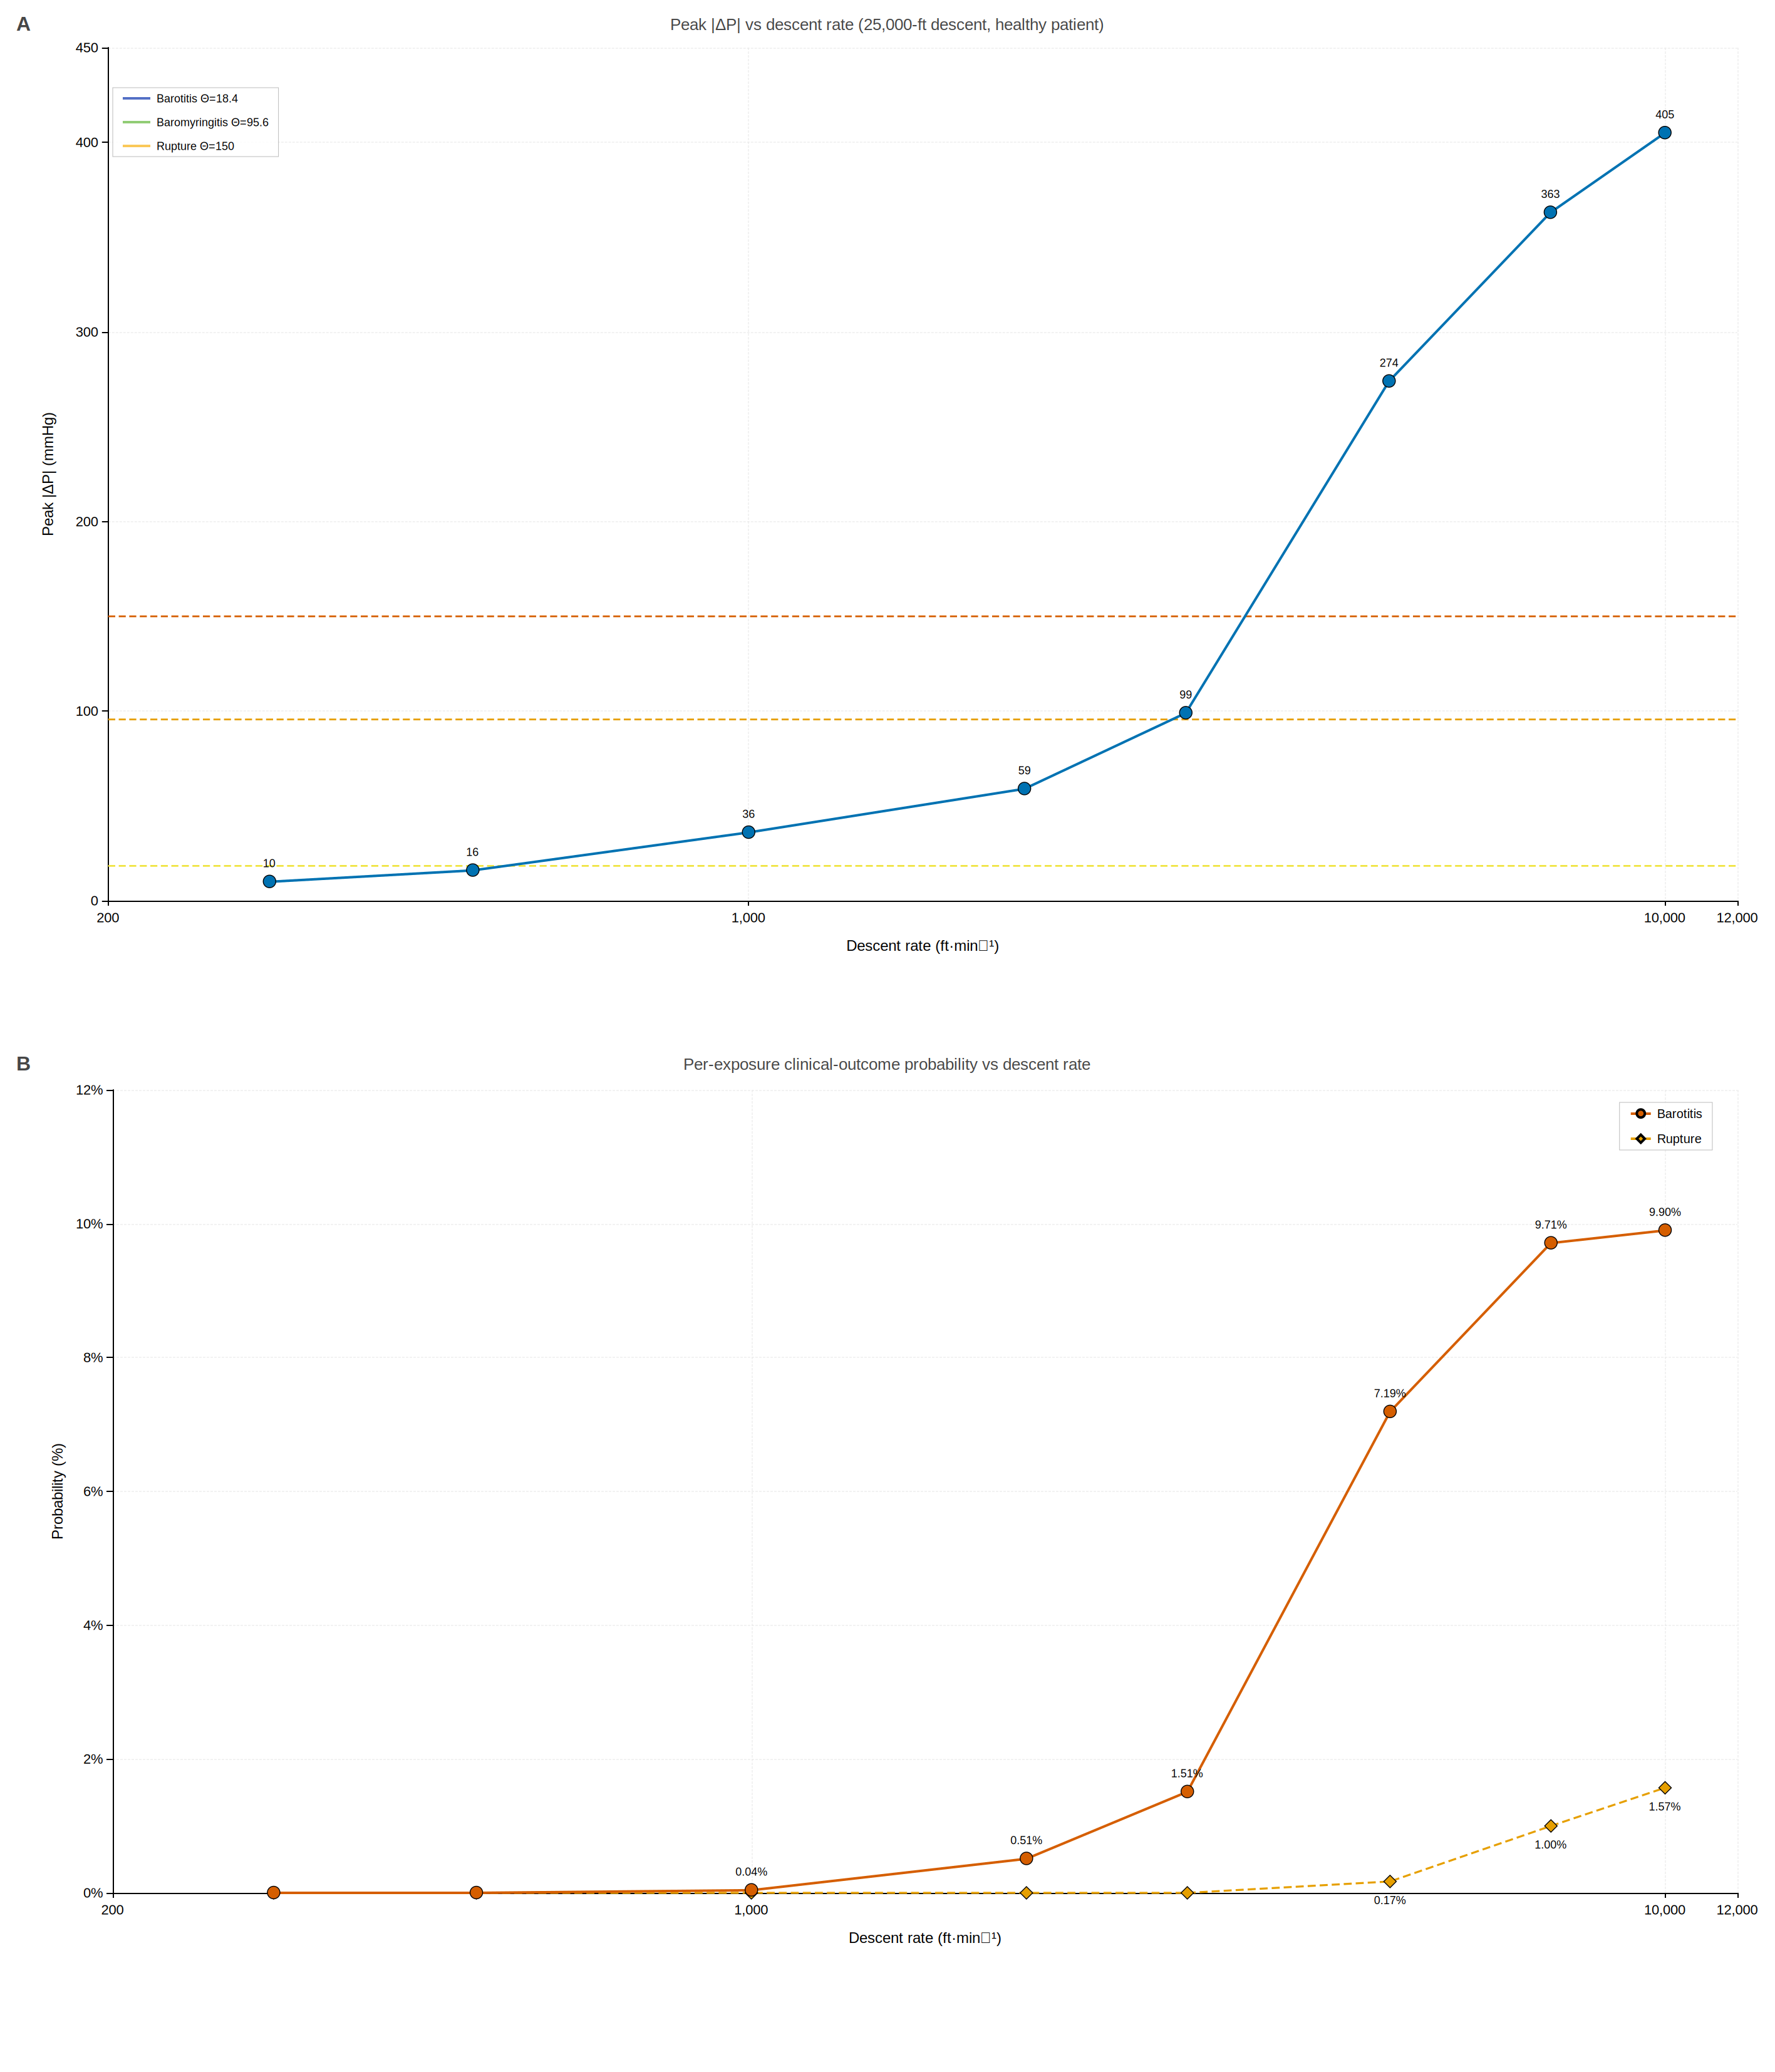
\includegraphics[width=0.85\textwidth]{../figures/paper_c/fig_01_descent_rate_sensitivity.png}
\caption{Descent-rate sensitivity for a healthy patient on a 25,000-ft descent. Peak $|\Delta P|$ (top panel) grows monotonically with descent rate, approaching $\sim$400~mmHg at 10,000~ft$\cdot$min$^{-1}$. Per-exposure barotitis probability (bottom panel) increases across the full 500--10,000~ft$\cdot$min$^{-1}$ range because the dose-time integral does not saturate as sharply as the peak}
\label{fig:descent_rate}
\end{figure}

\begin{figure}[htbp]
\centering
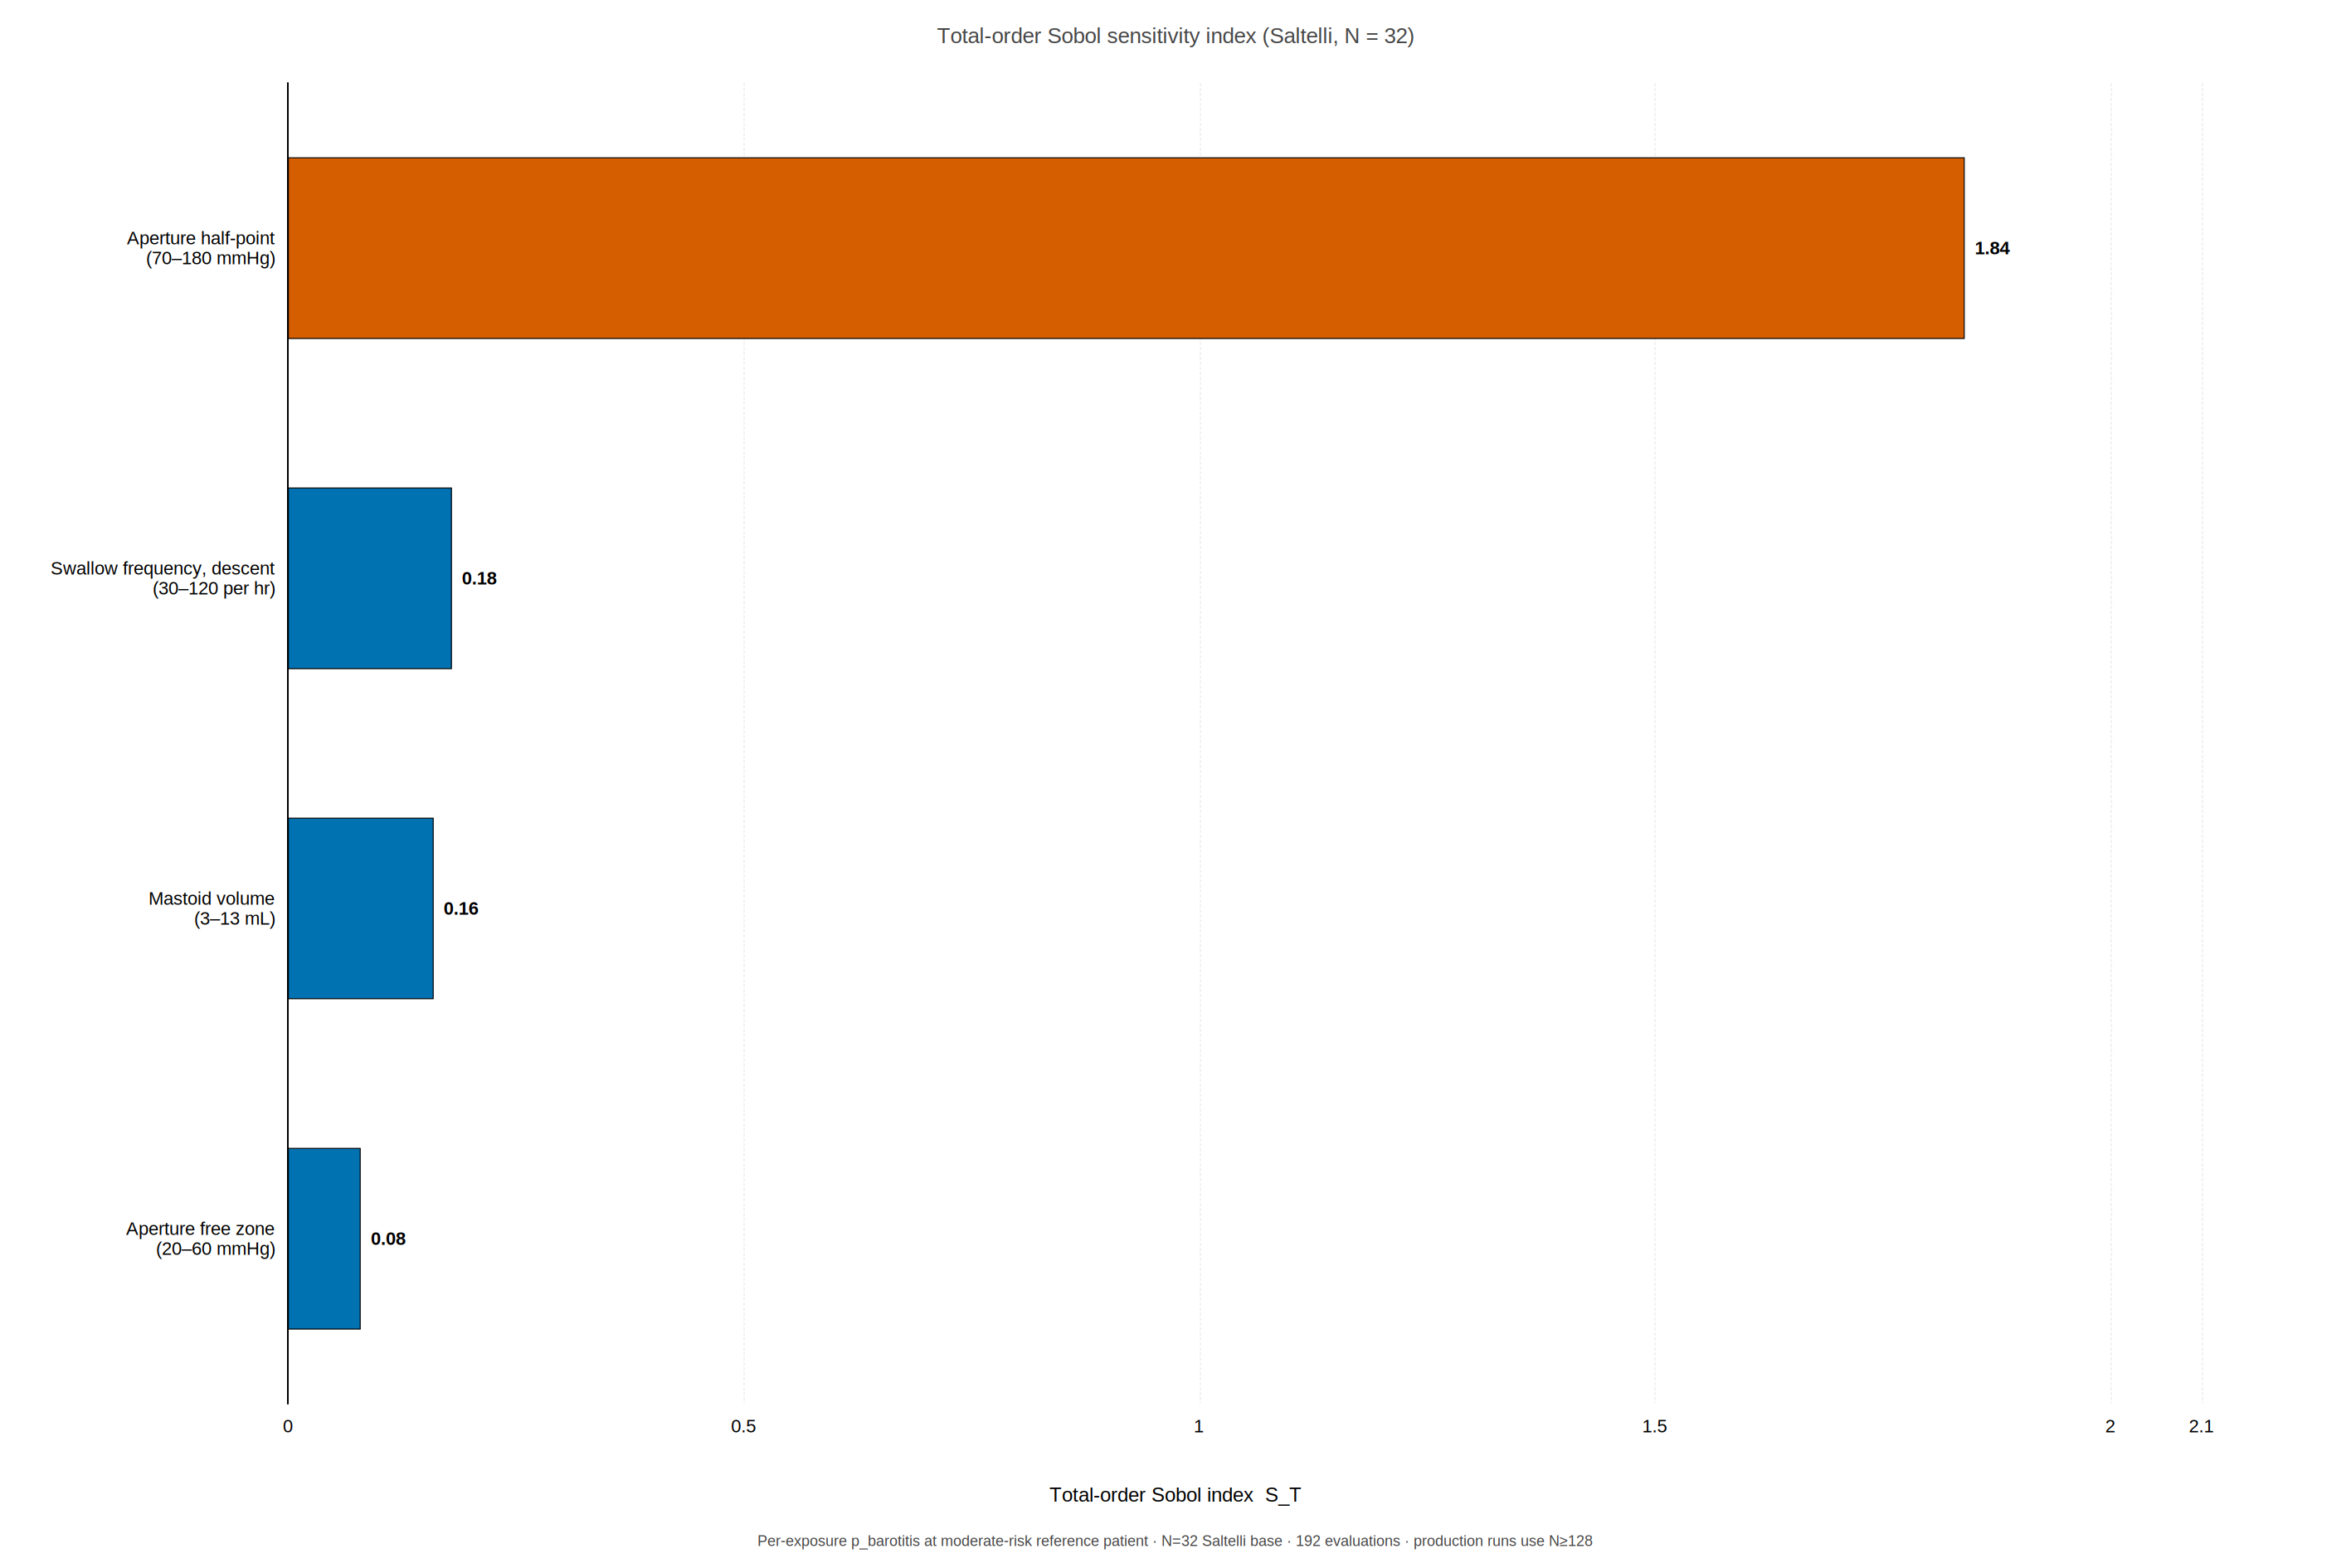
\includegraphics[width=0.85\textwidth]{../figures/paper_c/fig_02_sobol_sensitivity.png}
\caption{Saltelli-Sobol total-order sensitivity index over four model parameters evaluated at a moderate-risk reference patient ($N = 128$ Saltelli base samples; 768 model evaluations; scrambled-Sobol QMC sequence, seed~2026). The aperture half-point dominates ($S_T \approx 0.99$), approximately fifty-fold above descent-phase swallow frequency ($S_T = 0.020$), aperture free-zone threshold ($S_T = 0.019$), and mastoid volume ($S_T = 0.005$). The three secondary parameters are indistinguishable from each other within Monte-Carlo noise}
\label{fig:sobol}
\end{figure}

\begin{figure}[htbp]
\centering
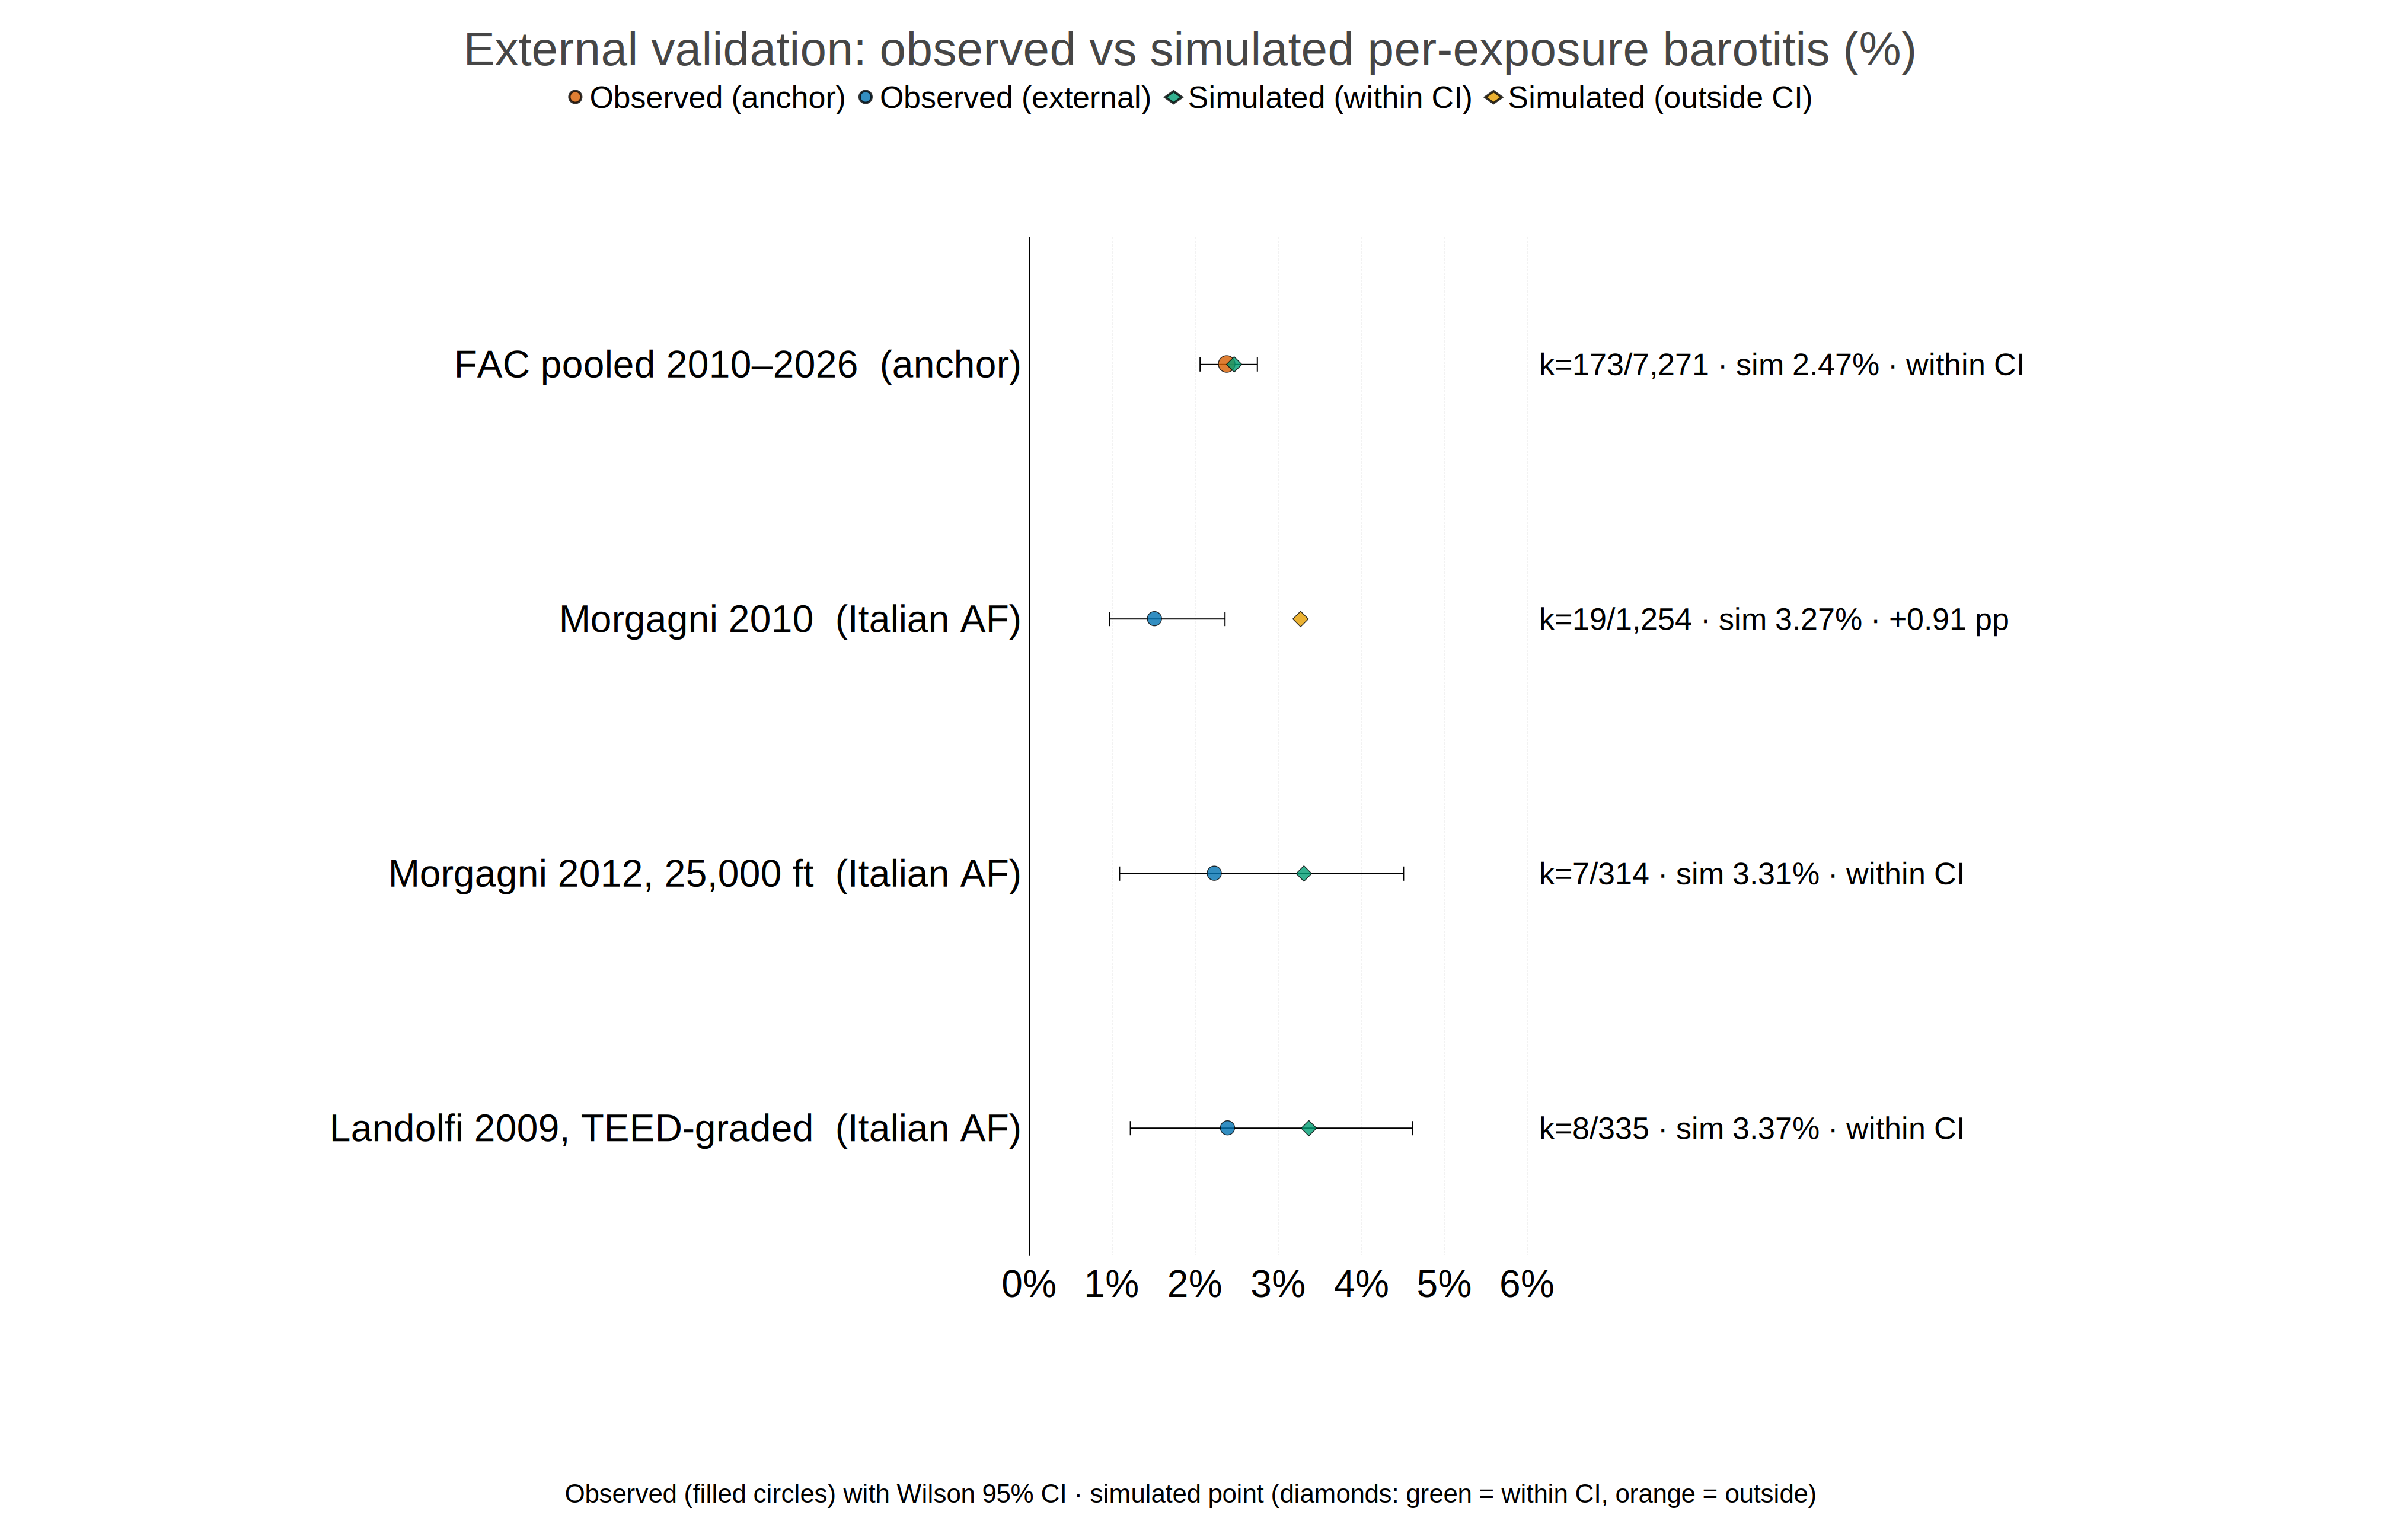
\includegraphics[width=0.85\textwidth]{../figures/paper_c/fig_03_external_validation.png}
\caption{External validation of the model against the calibration anchor (Colombian Aerospace Force pooled 2010--2026) and three independent previously published military-aviation cohorts (Morgagni 2010, Morgagni 2012, Landolfi 2009). Observed per-exposure barotitis incidence (filled circles) is shown with Wilson 95\% confidence intervals (whiskers); simulated point estimates (diamonds) are colored green when within the observed CI and orange when outside. The model fell within the observed CI for the calibration cohort (sim 2.47\% vs obs 2.38\%, CI [2.06--2.75]) and for two of the three external cohorts (Morgagni 2012 and Landolfi 2009). The Morgagni 2010 simulated point (3.27\%) sits 0.91 percentage points above the upper CI bound of that cohort's observed estimate (1.51\%, CI [0.97--2.36]), within the cohort's own pre-screened-to-unscreened denominator spread (1.1\% to 2.7\%) reported in the source publication. Right margin shows event count over cohort denominator and the simulated point with within-CI status}
\label{fig:validation}
\end{figure}

\begin{figure}[htbp]
\centering
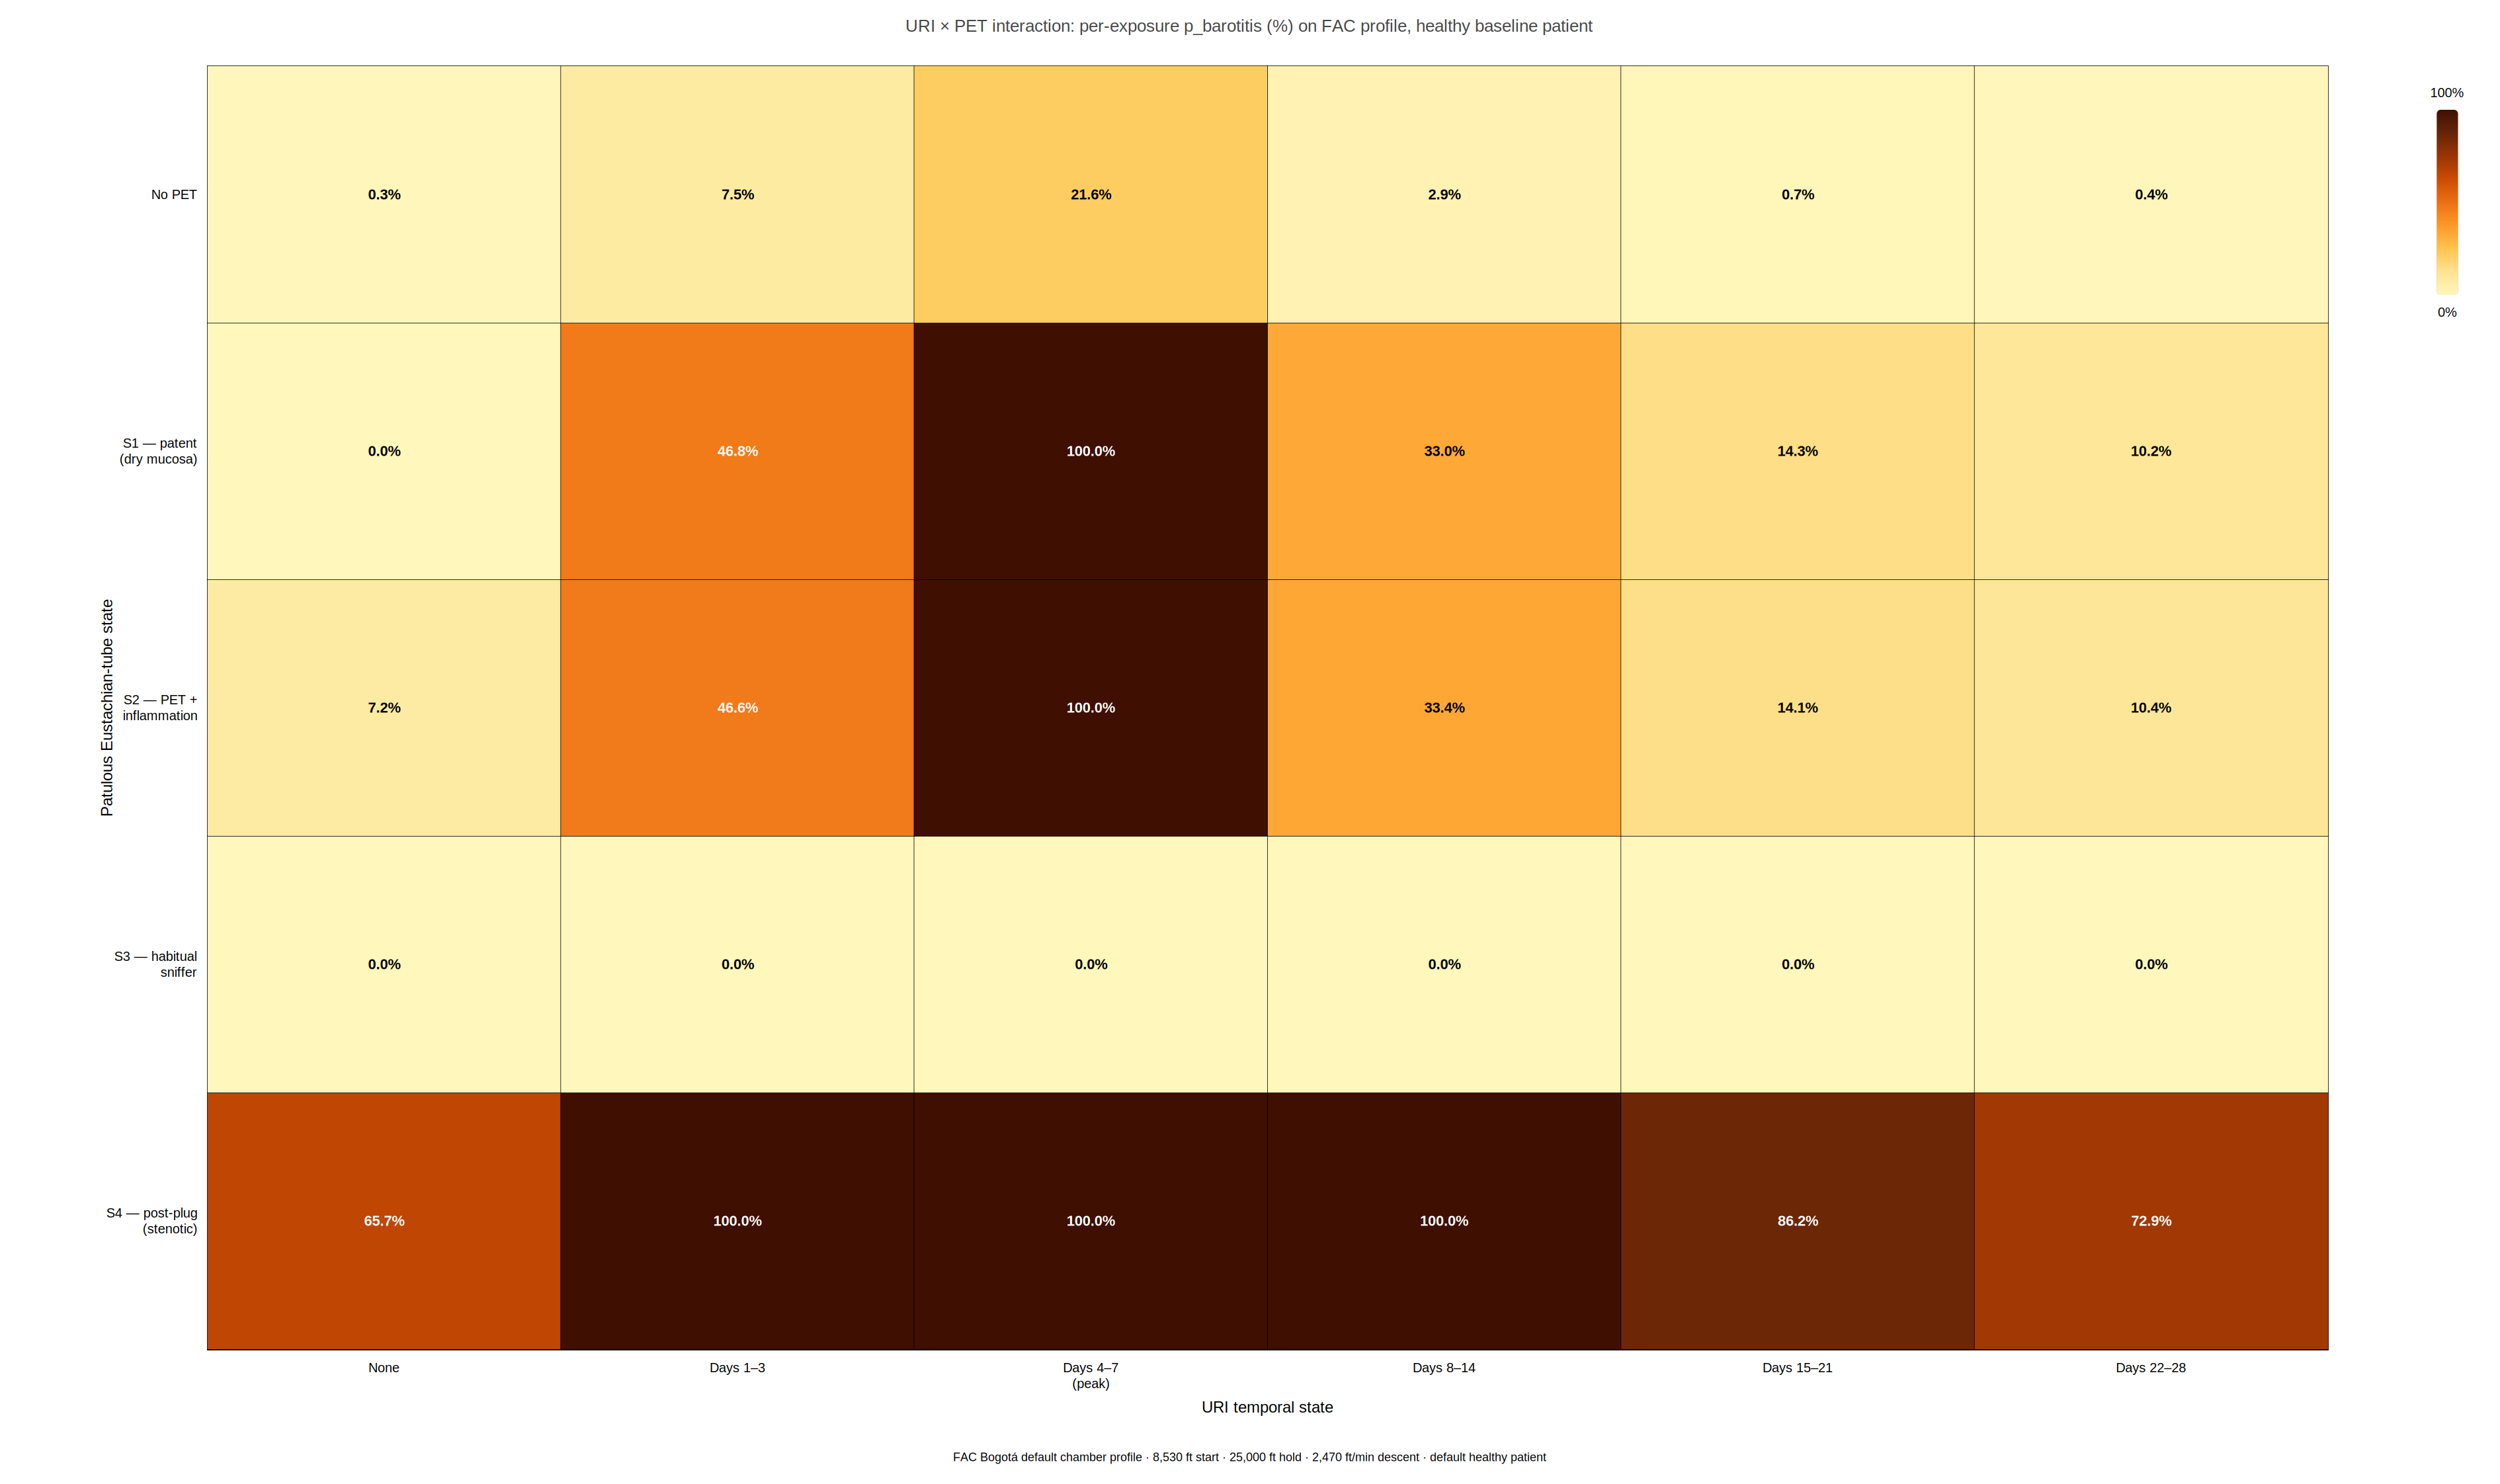
\includegraphics[width=0.85\textwidth]{../figures/paper_c/fig_04_uri_pet_interaction.png}
\caption{Joint dependence of per-exposure barotitis probability on Patulous Eustachian-tube state (5 levels: No PET, S1 baseline patent and dry mucosa, S2 PET with inflammation, S3 habitual sniffer, S4 post-Kobayashi plug or stenotic-equivalent) and upper-respiratory-infection temporal state (6 levels: none, days 1--3, 4--7, 8--14, 15--21, 22--28). Each cell is the model output for a default healthy baseline patient on the FAC Bogot\'{a} chamber profile (8,530~ft start, 25,000~ft hold, 2,470~ft$\cdot$min$^{-1}$ descent), varying only the URI and PET states; values were computed by \texttt{barotrauma.v2.simulate} over the full $5 \times 6$ grid. The peak-URI window (days 4--7) dominates each PET row. PET-S1 (rupture-protective in the original Kanick-Doyle 2005 binary treatment) is converted to high risk by URI exposure, matching the PET-with-inflammation pathophysiology in the Japan Otological Society criteria. PET-S4 saturates regardless of URI state. PET-S3 returns uniformly low risk on this profile because the negative resting-pressure bias offsets the descent-side $\Delta P$ integral; this model behavior is profile-specific and should not be interpreted as habitual sniffing being clinically protective}
\label{fig:uri_pet}
\end{figure}


% =====================================================================
% References
% =====================================================================

\bibliographystyle{apalike}
\bibliography{references}

\end{document}
